\begin{figure}[H]
\centering
    \resizebox{\linewidth}{!}{
    \subfloat["Taxi"]{
        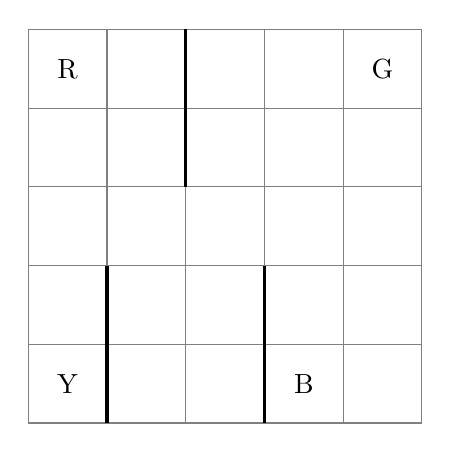
\begin{tikzpicture}
            \draw[step=1cm,color=gray] (0,0) grid (5,5);
            \node at (0.5,4.5) {R};
            \node at (4.5,4.5) {G};
            \node at (0.5,0.5) {Y};
            \node at (3.5,0.5) {B};
            \draw[very thick] (2,5) -- (2,3);
            \draw[very thick] (1,2) -- (1,0);
            \draw[very thick] (3,2) -- (3,0);
        \end{tikzpicture}}
    \qquad
    \subfloat["TaxiTraps"]{
        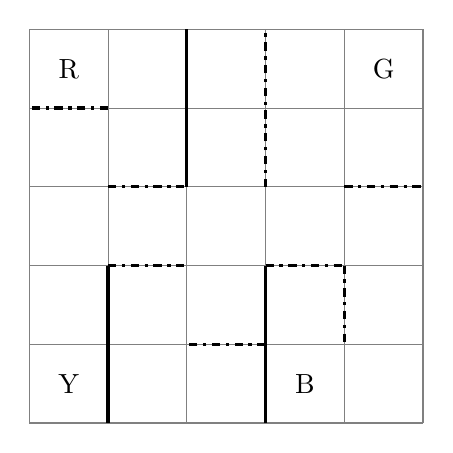
\begin{tikzpicture}
            \draw[step=1cm,color=gray] (0,0) grid (5,5);
            \node at (0.5,4.5) {R};
            \node at (4.5,4.5) {G};
            \node at (0.5,0.5) {Y};
            \node at (3.5,0.5) {B};
            \draw[very thick] (2,5) -- (2,3);
            \draw[very thick] (1,2) -- (1,0);
            \draw[very thick] (3,2) -- (3,0);
            \draw[very thick, dash dot] (1,4) -- (0,4);
            \draw[very thick, dash dot] (1,3) -- (2,3);
            \draw[very thick, dash dot] (3,1) -- (2,1);
            \draw[very thick, dash dot] (1,2) -- (2,2);
            \draw[very thick, dash dot] (3,2) -- (4,2);
            \draw[very thick, dash dot] (4,3) -- (5,3);
            \draw[very thick, dash dot] (3,3) -- (3,5);
            \draw[very thick, dash dot] (4,2) -- (4,1);
        \end{tikzpicture}}
    \qquad
    \subfloat["Taxi2"]{
        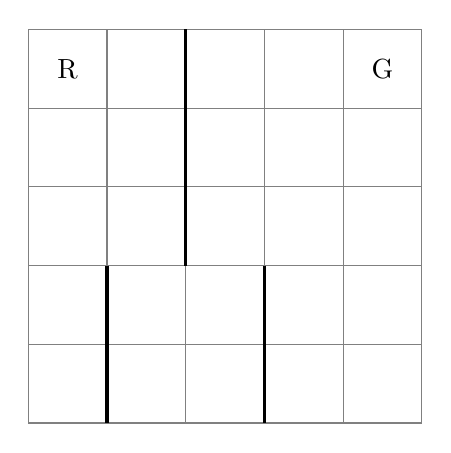
\begin{tikzpicture}
            \draw[step=1cm,color=gray] (0,0) grid (5,5);
            \node at (0.5,4.5) {R};
            \node at (4.5,4.5) {G};
            \draw[very thick] (2,5) -- (2,3);
            \draw[very thick] (1,2) -- (1,0);
            \draw[very thick] (3,2) -- (3,0);
            \draw[very thick] (2,3) -- (2,2);
        \end{tikzpicture}}}
    \caption{Original and modified 'Taxi' environments. The thick black lines represent the walls, while the dotted lines represent the "traps".}
    \label{fig:taxi}
\end{figure}